Se detallan las diferentes arquitecturas contenidas en los restantes tres archivos de la carpeta entrenarmodelos, estos archivos contienen diversos modelos propuestos:

\begin{itemize}

\item cnn\_tres.py: Crea los modelos de redes convolucionales propuestos con una arquitectura base de tres capas. Ver figura \ref{fig:uml9}.

\begin{figure}
	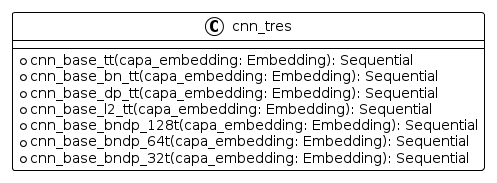
\includegraphics[width=0.65\textwidth]{capitulo5/figuras/fig9.png}
	\caption{Diagrama de clase del archivo cnn\_tres}
	\floatfoot{Fuente: Elaboración propia, generado con PlantUML}
	\label{fig:uml9}
\end{figure}

\item cnn\_four.py: Crea los modelos de redes convolucionales propuestos con una arquitectura base de cuatro capas. Ver figura \ref{fig:uml10}.

\begin{figure}
	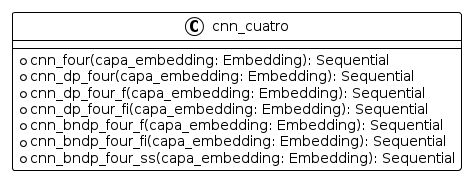
\includegraphics[width=0.65\textwidth]{capitulo5/figuras/fig10.png}
	\caption{Diagrama de clase del archivo cnn\_cuatro}
	\floatfoot{Fuente: Elaboración propia, generado con PlantUML}
	\label{fig:uml10}
\end{figure}

\item cnn\_dos.py: Crea los modelos de redes convolucionales propuestos con una arquitectura base de dos capas. Ver figura \ref{fig:uml11}.

\begin{figure}
	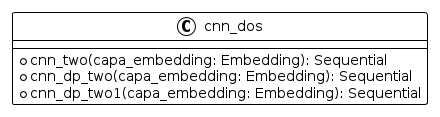
\includegraphics[width=0.65\textwidth]{capitulo5/figuras/fig11.png}
	\caption{Diagrama de clase del archivo cnn\_dos}
	\floatfoot{Fuente: Elaboración propia, generado con PlantUML}
	\label{fig:uml11}
\end{figure}

\end{itemize}

Para cada modelo propuesto, se guarda una copia en cualquier época durante el entrenamiento en la que la pérdida del conjunto de validación disminuya. Además, para mayor comodidad, se almacena todo el historial de entrenamiento de cada modelo, permitiendo visualizar su avance y realizar comparaciones con otros modelos.

